\documentclass[12pt,twoside]{article}

% *** Set page dimensions ***
\raggedbottom
\parindent=0in
%\setlength{\topmargin}{-0.5in}
%\setlength{\oddsidemargin}{0.1875in}
%\setlength{\evensidemargin}{0in}
%\setlength{\textheight}{8.5in}
%\setlength{\textwidth}{6.225in}
%\addtolength{\oddsidemargin}{-0.7in}
%\addtolength{\evensidemargin}{-1.2in}
%\setlength{\oddsidemargin}{-0.2in}
%\setlength{\evensidemargin}{-0.2in}
%\addtolength{\textwidth}{1.4in}
%\addtolength{\topmargin}{-.875in}
%\addtolength{\textheight}{2.00in}

% *** Packages ***
\usepackage{alltt}
\usepackage{tocloft}
\usepackage{graphicx}
\usepackage{lscape}
\usepackage{amssymb}
\usepackage{float}
\usepackage{amsmath}
\usepackage{gensymb}
%\usepackage{subfigure}
\usepackage{lscape}
\usepackage{epsfig}
\usepackage{enumerate}
\usepackage{multicol}
\usepackage{fancyhdr}
\usepackage{epstopdf}
\usepackage{hyperref}
\usepackage{listings}

% *** Table of contents and Sectioning *** 
\setcounter{secnumdepth}{0}
\setcounter{tocdepth}{5}

% *** Table of contents and Sectioning *** 
\newcommand{\next}{\addtocounter{enumi}{9} \item}
\newcommand{\now}[1]{\setcounter{enumi}{#1}}
\newcommand{\Z}{\mbox{\sf Z\hspace{-1.5mm}Z}}
\newcommand{\R}{\mbox{\rm I\hspace{-0.75mm}R}}
\columnsep=0.75in

% *** Shortcuts for syntax ***
\newcommand{\ds}{\displaystyle }
\newcommand{\vsc}{\vspace{4mm}}
\newcommand{\dd}[1]{\frac{d}{d{#1}} \,} 
\newcommand{\ddx}{\frac{d}{dx} \,} 
\newcommand{\ddy}{\frac{d}{dy} \,} 
\newcommand{\ddz}{\frac{d}{dz} \,} 
\newcommand{\dydx}{\frac{dy}{dx} \,} 
\newcommand{\dydt}{\frac{dy}{dt} \,} 
\newcommand{\dfdx}{\frac{df}{dx} \,} 
\newcommand{\ddt}[1]{  \frac{d{#1}}{dt} }
\newcommand{\pp}[2]{  \frac{\partial{#1}}{\partial {#2}} }
\newcommand{\zx}{\frac{\partial z}{\partial x} \,}
\newcommand{\zy}{\frac{\partial z}{\partial y} \,}
\newcommand{\limh}{\lim_{h \rightarrow 0} \;}
\newcommand{\diff}{\frac{d}{dx} \,}
\newcommand{\de}{\Delta}
\renewcommand{\thesection}{\Roman{section}}
\newcommand{\bfr}{\begin{flushright}}
\newcommand{\efr}{\end{flushright}}
\newcommand{\dx}{\frac{\partial f}{\partial x} \,}
\newcommand{\dy}{\frac{\partial f}{\partial y} \,}
\newcommand{\p}{\partial}
\newcommand{\vi}{\vec{i}}
\newcommand{\vj}{\vec{j}}
\newcommand{\vk}{\vec{k}}
\newcommand{\lan}{\left\langle}
\newcommand{\ran}{\right\rangle}
\newcommand{\reading}[1] { {\em Reading: #1}}
\renewcommand{\Pr}{ \mbox{Pr}}

% *** Commands related to textbook references
\newcommand{\problem}{{\bf Problem.} }

% *** Footnoting with symbols ***
\long\def\symbolfootnote[#1]#2{\begingroup%
\def\thefootnote{\fnsymbol{footnote}}\footnote[#1]{#2}\endgroup}

% *** Defining a boxed note ***
\floatstyle{boxed}
\newfloat{noteinbox}{htb}{loa}
\newenvironment{boxnote}{\begin{noteinbox}[H]}{\end{noteinbox}}

\newcommand{\Question}{ {\bf Question: }  }
\newcommand{\Example}[1]{ {\bf Example: } {\em #1} }
\newcommand{\ExampleCont}[1]{ {\em #1} }

% *** Define the boxed Week #/summary at the beginning/end of every chapter ***
\newcommand{\sectionbox}[1]{% 
\begin{tabular}{|p{6in}|}%
\hline%
\ \\ %
{\Large {\bf {#1}}}  \\%
\ \\%
\hline%
\end{tabular}}

% *** Shortcuts *** 
\newcommand\goals{\large {\bf {Goals:}}}
\newcommand\setfont{ }

% *** Week commands: overwritten in each notes file
\newcommand{\Week}{Null-InPreambleCommon}
\newcommand{\WeekTitle}{Null-InPreambleCommon}
\newcommand{\Course}{MNTC P04}
\newcommand{\SetNum}{1 }
\newcommand{\topic}[1]{
\newpage
\setcounter{page}{1}
\fancyhead[LE,RO]{#1 - \thepage}
}

% *** Setup Latex for the large version of the files ***
%\usepackage[landscape]{geometry}
\usepackage[letterpaper,landscape,hmargin={.8in,.8in},vmargin={1in,0.2in}]{geometry}

% Remove paragraph indents
\setlength{\parindent}{0pt}

% Spacing at the top for the header is too large by default
\setlength{\voffset}{-5ex}

% **** RENEW SCALING COMMANDS HERE ****
% *** Text in boxes ***
\renewenvironment{boxnote}{\begin{noteinbox}[H] \huge}{\end{noteinbox}} 

% *** Chapter lead in/summary boxes ***
\renewcommand{\sectionbox}[1]{% 
\begin{tabular}{|p{9.5in}|}%
\hline%
\ \\ %
{\huge {\bf {#1}}}  \\%
\ \\%
\hline%
\end{tabular}}

% *** 'Section'' commands, which are sometimes used for spacing
% From http://zoonek.free.fr/LaTeX/LaTeX_samples_section/0.html
\makeatletter
 \renewcommand\section{\@startsection {section}{1}{\z@}%
                                    {-3.5ex \@plus -1ex \@minus -.2ex}%
                                    {0.3ex \@plus.2ex}%
                                    {\setfont\bf}}

 \renewcommand\subsection{\@startsection {subsection}{1}{\z@}%
                                    {-3.5ex \@plus -1ex \@minus -.2ex}%
                                    {0.3ex \@plus.2ex}%
                                    {\setfont\bf}}

% *** 'Goals' should be larger in the overheads ***
\renewcommand\goals{\huge {\bf {Goals:}}}
\renewcommand\setfont{\huge }

\thispagestyle{empty}

\setfont 

\newcommand{\WeekTitleOne}{Derivatives - Foundations}
\newcommand{\WeekTitleTwo}{Derivatives - Linearization and Applications}
\newcommand{\WeekTitleThree}{Derivatives - Modeling}
\newcommand{\WeekTitleFour}{Integrals - Foundations}
\newcommand{\WeekTitleFive}{Integrals - Techniques}
\newcommand{\WeekTitleSix}{Integrals - Modeling}
\newcommand{\WeekTitleSeven}{Differential Equations - }
\newcommand{\WeekTitleEight}{Differential Equations - }
\newcommand{\WeekTitleNine}{Differential Equations - }
\newcommand{\WeekTitleTen}{Linear Algebra - }
\newcommand{\WeekTitleEleven}{Linear Algebra - }
\newcommand{\WeekTitleTwelve}{Linear Algebra - }



\begin{document}
\setfont
\pagestyle{fancy}
\renewcommand{\Week}{9 }
\renewcommand{\WeekTitle}{\WeekTitleNine }

\fancyhead[LE,RO]{Week \Week}  % default, usually only for first page
\fancyfoot{}
\sectionbox{Week \#\Week: \WeekTitle}


\vspace{5mm}
\goals
\begin{itemize}
\item Take problems that can be modeled by differential equations,
  both first and second order, and give solutions both by hand and
  MATLAB 
\item Examine case studies of differential equations applied to
  engineering problems and reproduce those solutions
\end{itemize}
\vspace{5mm}

%Falling body problem (maybe even the redbull stratos jump?)
%Electric Circuits
%Suspension cable bridge

\newpage

\topic{Application - Pendulum}
\subsection*{Application - Pendulum }
\begin{minipage}[t]{0.25\linewidth}
\vspace{0pt}
\begin{center}
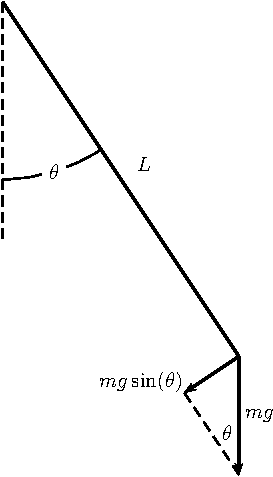
\includegraphics[width=1.0\linewidth]{graphics/notes_09_pendulum_diagram}
\end{center}
\end{minipage}
\begin{minipage}[t]{0.70\linewidth}
\vspace{0pt}
\begin{align*}
  \mbox{Newton's }& \mbox{ Second Law: } \\
   m  L^2 \theta'' & = T_g + T_f  \\
  & = - m L g \sin(\theta) - (\mu L^2 m) \theta' \\[3ex]
  \mbox{Solving for $\theta''$: }\theta'' & = - \frac{g}{L} \sin(\theta) - \mu 
  \theta'
\end{align*}
\end{minipage}

\problem Turn this single second-order DE into a pair of first-order
DEs.

\newpage
\problem Compare the system of differential equations we obtained to
the equations that define the motion of the damped spring/mass system.

\begin{minipage}[t]{0.45\linewidth}
\vspace{0pt}
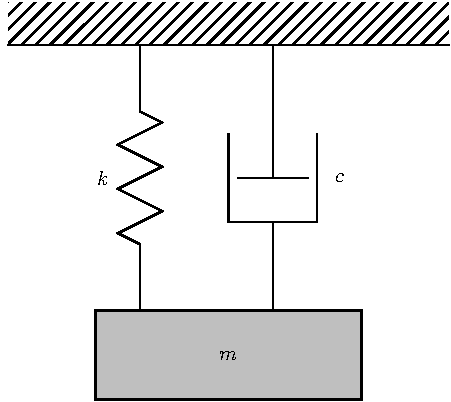
\includegraphics[width=0.4\linewidth]{graphics/notes_08_hanging_mass}
\begin{align*}
  \frac{dw_1}{dt} & = w_2 \\
  \frac{dw_2}{dt} & = \left(\frac{1}{m}\right) (- k w_1-c w_2)
\end{align*}
\end{minipage}
\begin{minipage}[t]{0.45\linewidth}
\vspace{0pt}
\begin{center}
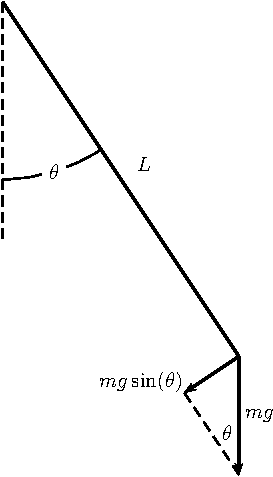
\includegraphics[width=0.2\linewidth]{graphics/notes_09_pendulum_diagram}
\end{center}
\begin{align*}
  \frac{d w_1}{dt} & = w_2 \\
  \frac{d w_2}{dt} & = -\frac{g}{L}\sin(w_1)  - \mu w_2
\end{align*}
\end{minipage}

\newpage


\problem Create a new MATLAB function file called \texttt{pendulumDE.m}.
Start with the first line
\begin{verbatim}
function dw_dt = pendulumDE(t, w, g, L, mu) 
\end{verbatim}

In the body of the function, implement the system of differential
equations 
\begin{align*}
  \frac{d w_1}{dt} & = w_2 \\
  \frac{d w_2}{dt} & = -\frac{g}{L}\sin(w_1)  - \mu w_2
\end{align*}
\vsc

\newpage

\problem Write a MATLAB script that simulates the motion of the
pendulum
using  \\
$g = 9.8$ m/s$^2$, $L$ = 2 m, $\mu = 0.1$, and \\
initial amplitude of 0.05 radians ($\approx 2.9$ degrees). \\
Generate a plot of the resulting angular position over time.


\newpage 
\topic{Pendulum - Period of Swings}
\subsection*{Pendulum - Period of Swings}

Galileo famously noticed the consistent period of pendulum swings,
even if the amplitude of the swings was changed (so the actual
distance travelled was different).

\vspace{2.5in}

\problem Compare the periods of the pendulum swings, using a range of
initial angles from $\theta_0 = 0.05$ radians up to $\theta_0 = 0.25$
radians ($\approx 14$ degrees).


\newpage
However, it turns out that pendulums are {\bf not} perfectly
consistent in their period, due to the non-linear term
$\ds -\frac{g}{L} \sin(\theta)$ in one of the forces: as the
amplitudes get bigger, there is a gradual lengthening of the period.


\problem Compare the periods of the pendulum swings, using a range of
initial angles from $\theta_0 = 0.25$ radians up to $\theta_0 = \frac{\pi}{2}$
radians ($= 90$ degrees).

\newpage

\problem Use these observations to explain the designs you see for
pendulum-based clocks.

\newpage

\topic{Pendulum -  Including an Initial Velocity}
\subsection*{Pendulum -  Including an Initial Velocity}

\problem Write a new simulation script that starts the pendulum
swinging from $ \theta_0 = -\frac{\pi}{2}$, with no initial velocity.
Simulate the motion for this scenario and generate a graph of the
angle against time.

Use the  parameters $g = 9.8$ m/s$^2$, $L$ = 2 m, and $\mu = 0.1$. \\

\vsc

\newpage

If we add a high enough initial `kick', or initial velocity, it would
be possible to make the mass of the pendulum go ``over the top'', or
above the point of rotation.

\problem Sketch what the anglular position graph would look like for
this scenario.

\newpage

\problem If we keep the initial angle at $-\frac{\pi}{2}$ (pendulum
out horizontally), experiment with the MATLAB code to find the initial
velocity that will push the pendulum ``over the top''.

\newpage

\topic{Application - Lake Mixing Model}
\subsection{Application - Lake Mixing Model}
Consider a small lake that initially contains $10$ million litres of
fresh water.  Water containing an undesirable chemical flows into the
lake at the rate of $5$ million litres per year; the mixture in the
lake flows out at the same rate.  The concentration $c(t)$ of chemical
in the incoming water varies periodically with time according to the
expression $c(t) = 2 + \sin(2t) \; \text{g} \cdot \text{L}^{-1}$.

  \problem Construct a mathematical model of this flow process.

\newpage
\problem Use MATLAB and a differential equation solver to determine
the amount of chemical in the lake over time, assuming that the lake
started without any contamination.

\newpage

\topic{Application - Tailings Pond With Sediment}
\subsection*{Application - Tailings Pond With Sediment}
% Source: http://faculty.sfasu.edu/judsontw/ode/html/firstlook05.html
Consider a tailings pond, where the the inflow contains both an
environmentally sensitive chemical, and sediments that will settle out
of the water.

\begin{itemize}
\item The volume of the pond is 40,000 cubic meters.
\item Water is flowing in and out of the pond at a rate of 1,500 cubic
  meters per day.
\item The water flowing into the pond contains 2 g of toxic chemical
  per cubic meter.
\item The inflow water also contains 1\% sediments
\end{itemize}

\problem Sketch a diagram of this scenario.

\newpage

\problem Write a differential equation that describes the rate of
change of the concentration of the chemical in the water remaining in
the tailings pond.

\newpage

\problem Use MATLAB and a differential equation solver to determine
the concentration of chemical in the water part of the tailings pond,
assuming that the pond started without any contamination.


\newpage

\problem Comment on any mismatch between the model and the reality
that should be addressed to make the model more accurate.

\newpage
\topic{Application - Interconnected Tanks}
\section*{Application- Interconnected Tanks}

\noindent
Consider the tanks shown below, which shows water flowing between the
tanks, and the concentration of a salt solution coming in.  Within
each tank, the water/salt solution is kept well mixed.
\begin{center}
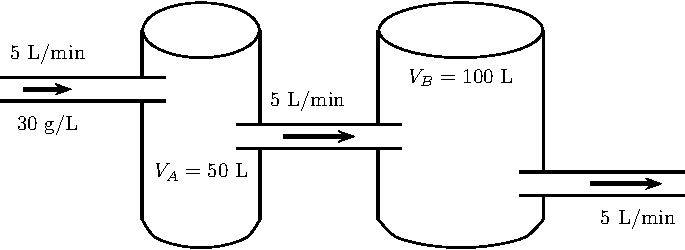
\includegraphics[width=0.7\linewidth]{graphics/notes_09_tanks1}
\end{center}

\begin{problem}
  If both tanks start with no salt, sketch what you expect will happen
  to the concentration within each tank over time.
\end{problem}

\newpage
\begin{minipage}[h]{0.5\linewidth}
\vspace{0pt}
\begin{problem}
Create a system of differential equations that dictate 
how the two tank concentrations will evolve over time.
\end{problem}
\end{minipage} \hfill
\begin{minipage}[h]{0.45\linewidth}
\vspace{0pt}
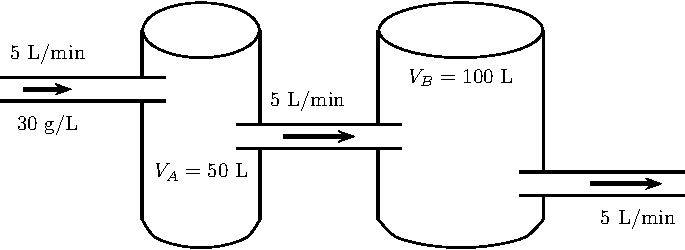
\includegraphics[width=1.0\linewidth]{graphics/notes_09_tanks1}
\end{minipage}


\newpage
\begin{minipage}[t]{0.5\linewidth}
\vspace{0pt}
\problem
  Use MATLAB and a differential equation solver to predict the exact salt concentrations over time
in {\bf both tanks}. 
% \begin{align*}
% \frac{dc_A}{dt}    & = \frac{-1}{10} c_A + 3; \\
% \frac{dc_B}{dt}    & = \frac{1}{20} c_A -\frac{1}{20} c_B 
% \end{align*}
\end{minipage}
\begin{minipage}[t]{0.45\linewidth}
\vspace{0pt}
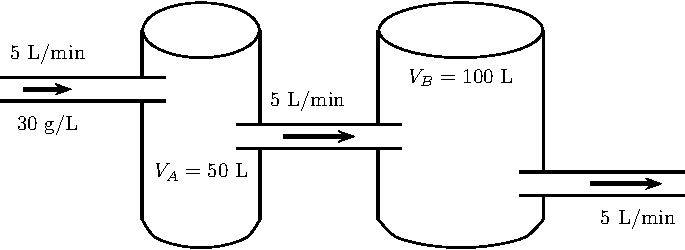
\includegraphics[width=1.0\linewidth]{graphics/notes_09_tanks1}
\end{minipage}

\newpage

\topic{Tank Model - Example 2}
\subsection*{Tank Model - Example 2}

Consider the more complicated tank arrangement shown below.
\begin{center}
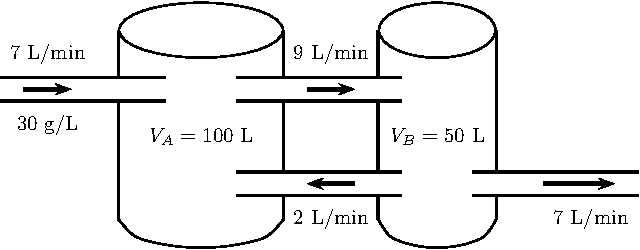
\includegraphics[width=0.7\linewidth]{graphics/notes_09_tanks2}
\end{center}
\begin{problem}
Given that the initial concentrations are \\
$c_A(0) = 0 $ g/L and $c_B(0)  = 90$ g/L,  \\
sketch what you would predict for the concentration in each tank over time.
\end{problem}

\newpage
\begin{minipage}[h]{0.5\linewidth}
\vspace{0pt}
\begin{problem}
  Construct the differential equation for the salt concentration in
  each tank.
\end{problem}
\end{minipage} \hfill
\begin{minipage}[h]{0.45\linewidth}
\vspace{0pt}
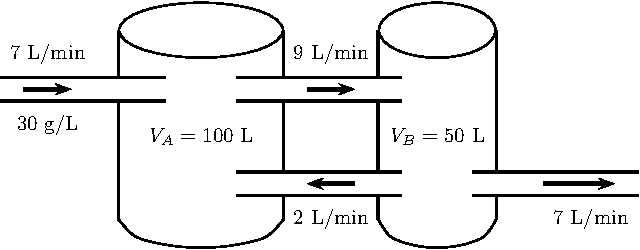
\includegraphics[width=1.0\linewidth]{graphics/notes_09_tanks2}
\end{minipage}

%\newpage
%\hfill 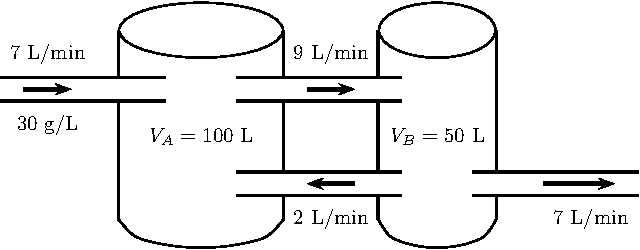
\includegraphics[width=0.5\linewidth]{graphics/notes_09_tanks2}

\newpage

\begin{minipage}[h]{0.5\linewidth}
  \vspace{0pt} \problem Use MATLAB and a differential equation solver
  to predict the salt concentrations over time by solving the system
  of differential equations
  \begin{align*}
    \frac{dc_A}{dt} & = -0.09 c_A + 0.02 c_B + 2.1 \\
    \frac{dc_B}{dt} & = 0.18 c_A - 0.18 c_B \\
  \end{align*}
\end{minipage} \hfill
\begin{minipage}[h]{0.45\linewidth}
\vspace{0pt}
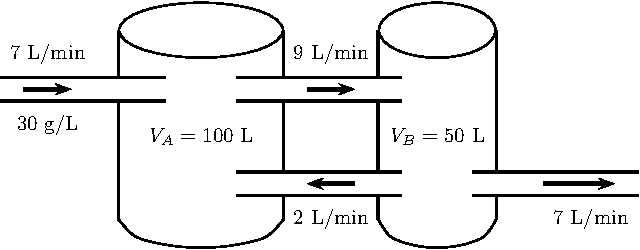
\includegraphics[width=1.0\linewidth]{graphics/notes_09_tanks2}
\end{minipage}


\newpage


~\hfill \begin{minipage}[h]{0.45\linewidth}
\vspace{0pt}
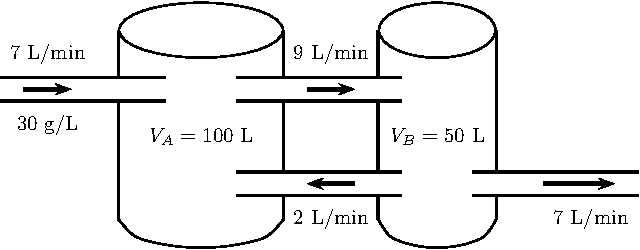
\includegraphics[width=1.0\linewidth]{graphics/notes_09_tanks2}
\end{minipage}



\end{document}
%Confirmation of deflection:
%  http://www.efunda.com/formulae/solid_mechanics/beams/casestudy_display.cfm?case=cantilever_uniformload


\end{document}

